\chapter{Balance and Equilibrium}\label{ch:g2:balance-equilibrium}

A seesaw hangs level with a child on each end. A tower of blocks
stands --- one block more, and it crashes. An acrobat walks a rope
thinner than her shoe. All three are playing the same deep game:
the game of balance, where \omterm{def:g2:pushes-and-pulls:force}{forces} cancel and nothing moves.

\section{Standing still is a balance}

\begin{definition}[Equilibrium]\label{def:g2:balance-equilibrium:equilibrium}
A thing is in \emph{equilibrium}\index{equilibrium} --- we also say
\emph{balanced}\index{balanced} --- when the pushes and pulls on it
cancel each other out, so it stays exactly as it is. The tug-of-war
ribbon standing still between two mighty teams: equilibrium. Not a
world without \omterm{def:g2:pushes-and-pulls:force}{forces} --- a world where the \omterm{def:g2:pushes-and-pulls:force}{forces} are having a
perfect tie.
\end{definition}

\begin{example}[The book on the table]\label{ex:g2:balance-equilibrium:book}
A book lies on the table, perfectly still. Boring? Look closer with
last chapter's eyes. The Earth pulls the book down --- so why does
it not fall? Because the table pushes it \emph{up}, exactly as hard
as the Earth pulls down. Two arrows, equal and opposite: a tie. Take
the table away and the tie is broken: down goes the book.
\end{example}

\begin{omfigure}
\begin{tikzpicture}[scale=0.85]
  \draw[thick] (0.4,1.2) -- (5.6,1.2);
  \draw[thick] (0.9,1.2) -- (0.9,0) (5.1,1.2) -- (5.1,0);
  \draw[thick, fill=omMeth, fill opacity=0.4]
    (2.2,1.2) rectangle (3.8,1.75);
  \node[font=\small] at (3.0,1.47) {book};
  \draw[-Stealth, very thick, omDef] (3.0,1.1) -- (3.0,0.25);
  \node[right, font=\small, omDef] at (3.15,0.6)
    {the Earth pulls down};
  \draw[-Stealth, very thick, omThm] (3.0,1.85) -- (3.0,2.7);
  \node[right, font=\small, omThm] at (3.15,2.4)
    {the table pushes up};
\end{tikzpicture}

{\small The stillest thing in the room is a perfect tie: two equal
arrows, opposite ways. \omterm{def:g2:balance-equilibrium:equilibrium}{Equilibrium}.}
\end{omfigure}

\begin{remark}[Still does not mean force-free]\label{rem:g2:balance-equilibrium:notfree}
Before this chapter, ``nothing is happening to the book'' seemed
obvious. Now you know better: two \omterm{def:g2:pushes-and-pulls:force}{forces} act on it every moment. All
around you, chairs, lamps, houses and mountains are held in quiet
ties of pulling and pushing. Stillness is not emptiness --- it is
balance.
\end{remark}

\section{The seesaw}

\begin{example}[A tie on the playground]\label{ex:g2:balance-equilibrium:seesaw}
Two friends of about the same size sit at the two ends of a seesaw:
it hangs level --- a tie. Now Papa sits on one end: down he goes,
and up flies the child. To play fair, Papa scoots \emph{toward the
middle}: the closer he sits to the pivot, the weaker his side
presses --- until, at just the right spot, the seesaw hangs level
again. A big weight near the middle can tie with a small weight far
out.
\end{example}

\begin{omfigure}
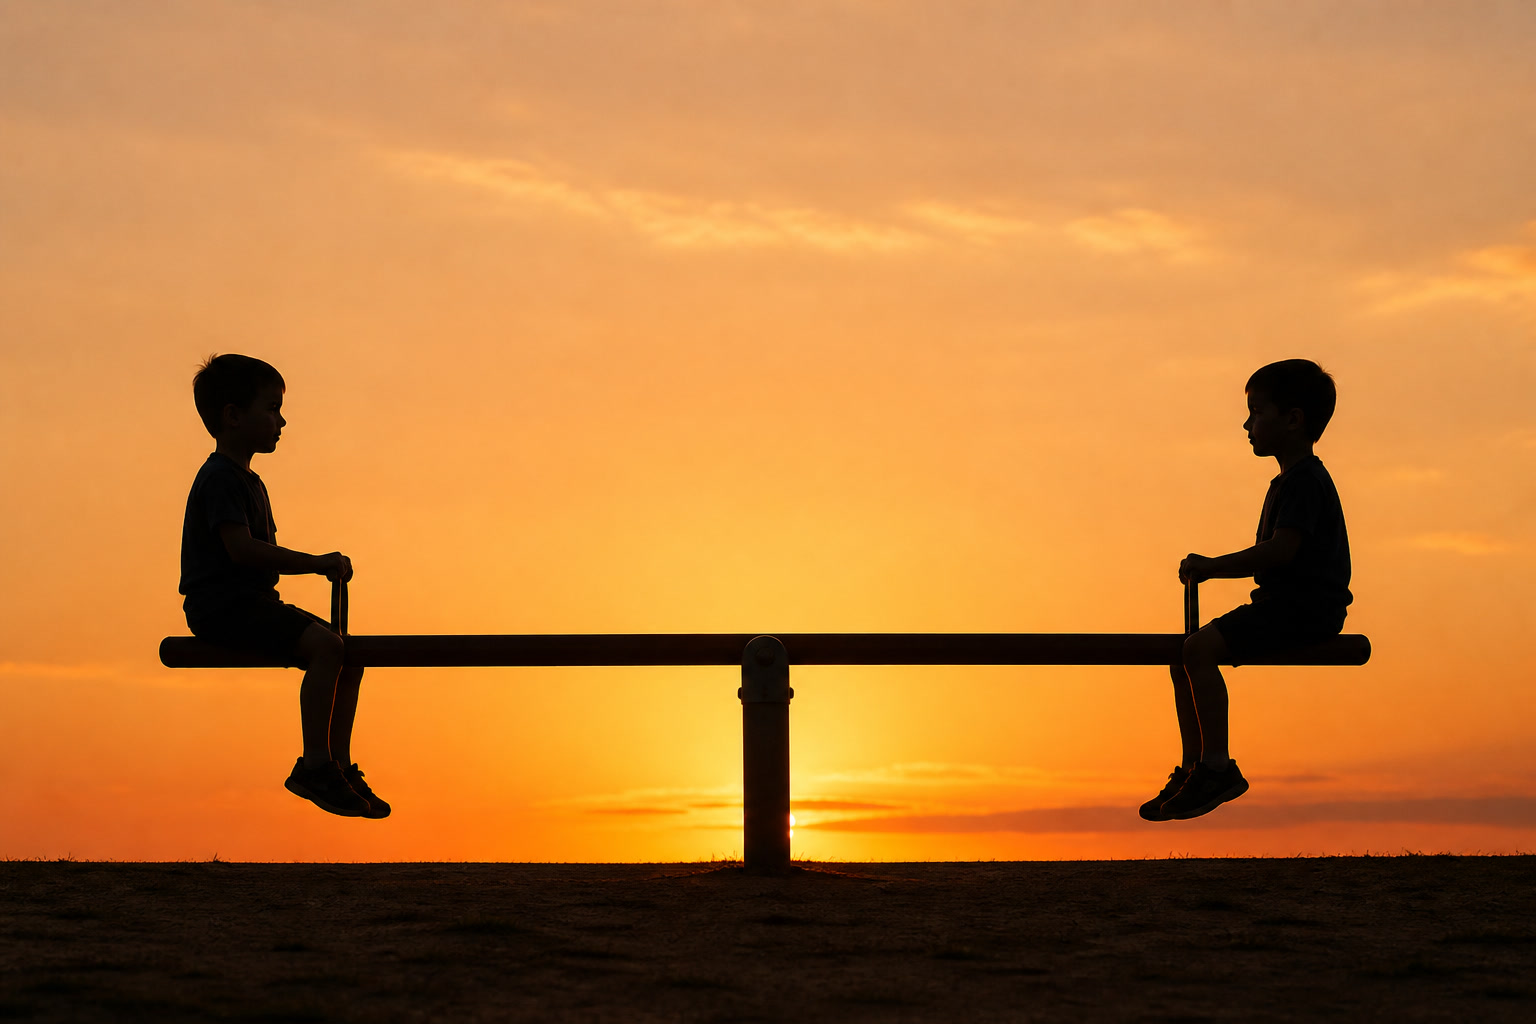
\includegraphics[width=0.58\linewidth]{images/book1/ai/g2-balance-seesaw.jpg}

{\small A perfect tie on the playground: two riders of the same size, the same distance out --- and the seesaw hangs level.}
\end{omfigure}

\begin{proposition}[The seesaw rule]\label{prop:g2:balance-equilibrium:rule}
Equal weights at equal distances from the pivot balance. A heavier
rider tips the seesaw --- unless the heavier rider moves closer to
the pivot, or the lighter one moves farther out. Weight \emph{and}
distance both count.
\end{proposition}

\begin{omfigure}
\begin{tikzpicture}[scale=0.85]
  \draw[thick, fill=omExo, fill opacity=0.3]
    (2.6,0) -- (3.0,0.75) -- (2.2,0.75) -- cycle;
  \draw[very thick] (0.2,0.8) -- (5.0,0.8);
  \fill[omDef] (0.55,1.1) circle (0.26);
  \fill[omDef] (4.65,1.1) circle (0.26);
  \node[below, font=\small, align=center] at (2.6,-0.25)
    {equal weights, equal distances:\\level};
  \draw[thick, fill=omExo, fill opacity=0.3]
    (8.9,0) -- (9.3,0.75) -- (8.5,0.75) -- cycle;
  \draw[very thick] (6.5,0.8) -- (11.3,0.8);
  \fill[omThm] (9.9,1.15) circle (0.4);
  \fill[omDef] (6.85,1.1) circle (0.26);
  \node[below, font=\small, align=center] at (8.9,-0.25)
    {the heavy rider sits close:\\level again};
\end{tikzpicture}

{\small Two ways to a tie: same weights at same distances --- or a
heavy rider near the pivot against a \omterm{def:g1:light-and-shadows:source}{light} rider far away.}
\end{omfigure}

\begin{remark}[A promise]\label{rem:g2:balance-equilibrium:promise}
How close must Papa scoot, exactly? There is a beautiful, precise
rule hiding in the seesaw --- with real numbers in it. It is waiting
for you next year, in the chapter on levers and scales; today's
seesaw games are its perfect training.
\end{remark}

\section{Toppling and the balance point}

\begin{example}[The tower that leaned too far]\label{ex:g2:balance-equilibrium:tower}
Build a tower of blocks, each block sticking out a little more than
the one below. It stands, it stands\dots\ and suddenly it crashes. A
leaning thing topples when it leans \emph{too far out} past its own
base. That is why a wide-based pyramid of blocks is so hard to knock
over, while a single tall column falls at a breath: broad feet make
steady towers.
\end{example}

\begin{definition}[Balance point]\label{def:g2:balance-equilibrium:point}
The \emph{balance point}\index{balance point} of an object is the
special spot where it can be held up level --- as if all its weight
gathered there. A ruler carries its balance point in the middle; a
hammer hides it near the heavy head. Held right under its balance
point, any object rests level on one finger.
\end{definition}

\begin{method}[Finding the balance point]\label{met:g2:balance-equilibrium:find}
To find the \omterm{def:g2:balance-equilibrium:point}{balance point} of a ruler, a broom, or a wooden spoon:
\begin{enumerate}
  \item rest it across two stretched index fingers, one near each
        end;
  \item slide your fingers slowly toward each other;
  \item they will meet --- always with the object still \omterm{def:g2:balance-equilibrium:equilibrium}{balanced} ---
        at one spot: the \omterm{def:g2:balance-equilibrium:point}{balance point}.
\end{enumerate}
Try the broom: your fingers meet far from the middle, on the side of
the heavy brush. The \omterm{def:g2:balance-equilibrium:point}{balance point} loves the heavy side.
\end{method}

\begin{omfigure}
\begin{tikzpicture}[scale=0.85]
  \draw[thick, fill=omMeth, fill opacity=0.4]
    (0.3,1.5) rectangle (6.3,1.78);
  \draw[thick] (1.1,0.6) -- (1.1,1.45) (5.5,0.6) -- (5.5,1.45);
  \draw[-Stealth, omExo, thick] (1.45,0.9) -- (2.6,0.9);
  \draw[-Stealth, omExo, thick] (5.15,0.9) -- (4.0,0.9);
  \node[below, font=\small] at (3.3,0.45)
    {slide both fingers inward\dots};
  \draw[thick, fill=omMeth, fill opacity=0.4]
    (7.6,1.5) rectangle (11.6,1.78);
  \draw[thick] (9.6,0.6) -- (9.6,1.45);
  \fill[omThm] (9.6,1.92) circle (2.2pt);
  \node[below, font=\small] at (9.6,0.45)
    {\dots{}they meet under the balance point};
\end{tikzpicture}

{\small The two-finger trick: the sliding fingers always end up
right beneath the \omterm{def:g2:balance-equilibrium:point}{balance point}.}
\end{omfigure}

\begin{example}[The acrobat's pole]\label{ex:g2:balance-equilibrium:acrobat}
Why does the tightrope walker carry that long, drooping pole? It is
her balance helper: when she starts tipping to one side, the long
pole makes the lean slow and lazy instead of quick, and gives her
time to shift back over the rope. You use the same trick with bare
arms when you walk along a curb --- arms out, wobble slowed, balance
saved.
\end{example}

\section{Exercises}

\begin{exercise}[$\star$]\label{exo:g2:balance-equilibrium:1}
A lamp stands still on the desk. Name the two \omterm{def:g2:pushes-and-pulls:force}{forces} acting on it
and say why it does not move.
\end{exercise}

\begin{exercise}[$\star$]\label{exo:g2:balance-equilibrium:2}
In tug-of-war, when is the ribbon in \omterm{def:g2:balance-equilibrium:equilibrium}{equilibrium}? What breaks the
tie?
\end{exercise}

\begin{exercise}[$\star$]\label{exo:g2:balance-equilibrium:3}
Two equal twins sit on a seesaw at equal distances. What does the
seesaw do? One twin scoots backward, farther from the pivot ---
which side goes down now?
\end{exercise}

\begin{exercise}[$\star$]\label{exo:g2:balance-equilibrium:4}
Papa is much heavier than Lina, yet their seesaw hangs level. Where
must Papa be sitting? State the rule that saves the game.
\end{exercise}

\begin{exercise}[$\star$]\label{exo:g2:balance-equilibrium:5}
Where is the \omterm{def:g2:balance-equilibrium:point}{balance point} of a ruler? And of a hammer --- toward
the handle's end or the heavy head? How could you check with one
finger?
\end{exercise}

\begin{exercise}[$\star$]\label{exo:g2:balance-equilibrium:6}
Do the two-finger trick of \cref{met:g2:balance-equilibrium:find}
with a broom. On which side do your fingers meet, and what does
that tell you?
\end{exercise}

\begin{exercise}[$\star$]\label{exo:g2:balance-equilibrium:7}
Which stands more steadily, and why: a pyramid of blocks with a wide
bottom, or a one-block-wide tower of the same height?
\end{exercise}

\begin{exercise}[$\star$]\label{exo:g2:balance-equilibrium:8}
Why does a tightrope walker carry a long pole? What do you do with
your arms when you walk along a curb, and why does it help?
\end{exercise}

\begin{exercise}[$\star$]\label{exo:g2:balance-equilibrium:9}
Stand with your right shoulder and right foot pressed against a
wall, and try to lift your left foot. You cannot --- without
falling! Explain with the tower of
\cref{ex:g2:balance-equilibrium:tower}: what would your body have to
do to balance on the right foot, and what does the wall forbid?
\end{exercise}

\begin{exercise}[$\star\star$]\label{exo:g2:balance-equilibrium:10}
A crane on a building site lifts heavy loads on its long front arm
--- yet it does not tip over. On its short back arm sit huge
concrete blocks. Explain the crane with the seesaw rule of
\cref{prop:g2:balance-equilibrium:rule}: what are the two riders,
and why is the back arm short?
\end{exercise}
